\chapter{Parabolic Encounters Of A Massive Black Hole}

\section{Background \& Introduction}

Currently it is understood that many, if not all, galactic nuclei harboured a black hole at some point.\cite{Lynden-Bell1971, Rees1984}. The best opportunity to study these objects comes from the compact object in our own galactic centre, which is coincident with Sagittarius A* (Sgr A*). This is identified as a massive black hole (MBH) of mass $M_\bullet = \num{4.31e6} M_\odot$ and a distance of only $R_0 = \SI{8.88}{\kilo\parsec}$\cite{Gillessen2009}. According to the no-hair theorem the MBH should be described completely by its mass $M_\bullet$ and spin $a$ (since we expect  the charge of an astrophysical black hole to be negligible)\cite{Israel1967, Israel1968, Carter1971, Hawking1972, Robinson1975, Chandrasekhar1998}. Consequently, measuring the spin is necessary to fully understand the MBH and its role in the evolution of the Galaxy. It has been suggested that the spin could be inferred from careful observation of the orbits of stars within a few milliparsecs of the Galactic centre\cite{Merritt2010}, although this is complicated because of perturbations due to other stars, or from observations of quasi-periodic oscillations (QPOs) of radio emissions\cite{Kato2010}. This latter method has produced a value of the dimensionless spin, $a_\ast = Jc/GM_\bullet^2$ where $J$ is the MBH's angular momentum, of $a_\ast = 0.44 \pm 0.08$. However, to obtain this result Kato {\it et al.}\cite{Kato2010} have combined their observations of Sgr A* with observations of galactic X-ray sources containing solar mass BHs, to find a best-fit unique spin parameter for all BHs. This is somewhat unsatisfactory since it is not clear that all BHs should share the same value of the spin parameter; especially considering that the BHs considered here differ by six orders of magnitude, with none in the intermediate range. Even if BH spin is determined by a universal process, we would expect some distribution of spin parameters\cite{King2008}. Thus we cannot accurately determine the spin of the galactic centre's MBH from an average including other BHs. While we can use the spin of other BHs as a prior, to inform us of what we should expect to measure for the MBH's spin, it is desirable to have an independent measurement.

An exciting means of inferring information about the Galactic MBH is through gravitational waves (GWs) emitted when compact objects (COs), such as smaller BHs, neutron stars (NSs), white dwarfs (WDs) or low mass main sequence (MS) stars, pass close by. The planned LISA mission is designed to be able to detect GWs in the frequency range of interest for these encounters\cite{Bender1998, Danzmann2003}. The identification of waves requires a set of accurate waveform templates covering parameter space. Much work has already been done on the waveforms generated when companion objects inspiral towards an MBH; as they orbit, the GWs carry away energy and angular momentum, causing the orbit to shrink until eventually the object plunges into the MBH. The initial orbits may be highly elliptical and a burst of radiation is emitted during each close encounter. These are known as extreme mass-ratio bursts (EMRBs)\cite{Rubbo2006}. Assuming that the companion is not scattered from its orbit, and does not plunge straight into the MBH, its orbit will evolve, becoming more circular, and it will begin to emit continuously significant gravitational radiation in the LISA frequency range. The resulting signals are known as extreme mass-ratio inspirals (EMRIs).

Studies of these systems have usually focused upon when the orbit completes multiple cycles, thus allowing a high signal-to-noise ratio to be accumulated. Here, we will investigate what can be learnt from high eccentricity orbits. These are the initial orbits onto which we expect that COs may be scattered by interactions with other bodies. The event rate for the detection of such EMRBs with LISA has been estimated to be as high as $\SI{15}{\yr^{-1}}$\cite{Rubbo2006}, although this has been revised downwards to the order of $\SI{1}{\yr^{-1}}$\cite{Hopman2007}. Even if only a single burst is detected during the LISA mission, this is still an exciting possibility since the information carried by the GW should give an unparalleled probe of the structure of spacetime of the galactic centre. Exactly what can be inferred will depend upon the orbit.

We will make the simplifying assumption that all these orbits are marginally bound, or parabolic, since highly eccentric orbits will appear almost indistinguishable from an appropriate parabolic orbit\cite{Kobayashi2004}. Here ``parabolic'' and ``eccentricity'' refer to the energy of the geodesic and not to the geometric shape of the orbit.\footnote{Marginally bound Keplerian orbits in flat spacetime are parabolic in both senses.} Following such a trajectory an object may make just one pass of the MBH or, if the periapsis distance is small enough, it may complete a number or rotations. Such an orbit is referred to as zoom-whirl.

In order to compute the gravitational waveform produced in such a case, we integrate the geodesic equations for a parabolic orbit in Kerr spacetime. We assume that the orbiting body is a test particle, such that it does not influence the underlying spacetime, and that the orbital parameters evolve negligibly during the orbit so that they may be held constant. We use this to construct an approximate numerical kludge waveform\cite{Babak2007}.

\section{Parabolic Orbits in Kerr Spacetime}

\subsection{The Metric \& Geodesic Equations}

Astrophysical BHs are described by the Kerr metric\cite{Kerr1963}. In standard Boyer-Lindquist coordinates the line element is\cite{Boyer1967, Hobson2006}
\begin{equation}
\dd s^2 = \frac{\rho^2 \Delta}{\Sigma^2}c^2\dd t^2 - \frac{\Sigma \sin^2 \theta}{\rho^2}\left(\dd \phi - \omega \dd t\right)^2 - \frac{\rho^2}{\Delta}\dd r^2 - \rho^2\dd \theta^2,
\end{equation}
where we have introduced functions
\begin{align}
\rho^2 = {} & r^2 + a^2\cos^2\theta,\\
\Delta = {} & r^2 - \frac{2GM_\bullet r}{c^2} + a^2,\\
\Sigma = {} & \left(r^2 +a^2\right)^2 - a^2\Delta\sin^2\theta,\\
\omega = {} & \frac{2GM_\bullet ar}{c\Sigma}.
\end{align}
The spin parameter is related to the BH's angular momentum by
\begin{equation}
J = M_\bullet ac.
\end{equation}
For the remainder of this section we shall work in natural units with $G = c = 1$.

Geodesics are parameterized by three conserved quantities (aside from the particle's mass $\mu$): the energy (per unit mass) $E$, the specific angular momentum about the symmetry axis (the $z$-axis) $L_z$, and Carter constant $Q$\cite{Carter1968, Chandrasekhar1998}. The geodesic equations are
\begin{align}
\rho^2 \diff{t}{\tau} = {} & a\left(L_z - aE z\sin^2 \theta\right) + \frac{r^2 + a^2}{\Delta}T,\\
\rho^2 \diff{r}{\tau} = {} & \pm \sqrt{V_r},\\
\rho^2 \diff{\theta}{\tau} = {} & \pm \sqrt{V_\theta},\\
\rho^2 \diff{\phi}{\tau} = {} & \frac{L_z}{\sin^2 \theta} - aE + \frac{a}{\Delta}T,\\
\end{align}
where we have introduced potentials
\begin{align}
T = {} & E\left(r^2 +a^2\right) - aL_z,\\
V_r = {} & T^2 - \Delta\left[r^2 + \left(L_z -aE\right)^2 + Q\right],\\
V_\theta = {} & Q - \cos^2 \theta\left[a^2\left(1 - E^2\right) + \frac{L_z^2}{\sin^2\theta}\right],
\end{align}
and $\tau$ is proper time. The signs of the $r$ and $\theta$ equations may be chosen independently.

For a parabolic orbit $E = 1$, thus the particle is at rest at infinity. This simplifies the geodesic equations. It also allows us to give a simple interpretation for Carter constant $Q$: this is defined such that
\begin{equation}
Q = L_\theta^2 + \cos^2\theta\left[a^2\left(1 - E^2\right) + \frac{L_z^2}{\sin^2\theta}\right],
\end{equation}
where $L_\theta$ is the (non-conserved) specific angular momentum in the $\theta$ direction (note $L_\theta^2 = V_\theta$). For $E = 1$ we have
\begin{align}
Q = {} & L_\theta^2 + \cot^2\theta\, L_z^2 \nonumber \\
 = {} & L_\infty^2 - L_z^2
\end{align}
where $L_\infty$ is the total specific angular momentum at infinity, where the metric is asymptotically flat\cite{DeFelice1980}.\footnote{See Rosquist, Bylund \& Samuelsson\cite{Rosquist2009} for an interesting discussion of the interpretation of $Q$ in the limit $G \rightarrow 0$ corresponding to a flat spacetime.} This is just as in the Schwarzschild case.

\subsection{Integration Variables \& Turning Points}

In integrating the geodesic equations difficulties can arise because of the presence of turning points in the motion, when the sign of the $r$ or $\theta$ geodesic equation will change. The radial turning points are at the periapsis $r\sub{p}$ and at infinity. We may find the location of the periapsis by finding the roots of
\begin{align}
V_r = {} & 0 \nonumber \\
2M_\bullet r^3 - \left(L_z^2+Q\right)r^2 + 2M_\bullet\left[\left(L_z - a\right)^2 + Q\right]r - a^2Q = {} & 0.
\end{align}
This has three roots, which we shall denote $\{r_1, r_2, r\sub{p}\}$; the periapsis $r\sub{p}$ is the largest real root. We do not find the apoapsis as a (fourth) root to this equation as we have removed it by taking $E = 1$ before solving: it is simple to show this is a turning point by setting the unconstrained expression for $V_r$ equal to zero, and then solving for $E(r)$; taking the limit $r \rightarrow \infty$ gives $E \rightarrow 1$, so parabolic orbits do have a stationary point at infinity\cite{Wilkins1972}. We may avoid the difficulties of the turning point by introducing an angular variable that always increases with proper time\cite{Drasco2004}: inspired by Keplerian orbits, we may parameterize our parabolic trajectory by
\begin{equation}
r = \frac{p}{1+e\cos\psi},
\end{equation}
where $e = 1$ is the eccentricity and $p = 2r\sub{p}$ is the semilatus rectum. As $\psi$ covers its full range from $-\pi$ to $\pi$, $r$ traces out one full orbit from infinity through the periapsis at $\psi = 0$ back to infinity. The geodesic equation for $\psi$ is
\begin{equation}
\rho^2 \diff{\psi}{\tau} = \left\{M_\bullet\left[2r\sub{p} - \left(r_1 + r_2\right)\left(1 + \cos\psi\right) + \frac{r_1 r_2}{2r\sub{p}}\left(1 + \cos\psi\right)^2\right]\right\}^{1/2}.
\end{equation}
This may be integrated without problem. Parameterizing an orbit by its periapsis and eccentricity has the additional benefit of allowing easier comparison with its flat-space equivalent than considering energy and angular momentum\cite{Gair2005}.

The $\theta$ motion is usually bounded, with $\theta_0 \leq \theta \leq \pi - \theta_0$; in the event that $L_z = 0$ the particle follows a polar orbit and $\theta$ will cover its full range. The turning points are given by
\begin{align}
V_\theta = {} & 0 \nonumber \\
Q - \cot^2\theta\, L_z^2= {} & 0.
\end{align}
Note that only if $L_z = 0$ may we reach the poles\cite{Wilkins1972}. If we change variable to $\zeta = \cos^2\theta$, we have a maximum value $\zeta_0 = \cos^2\theta_0$ given by
\begin{align}
\label{eq:theta_0}
\zeta_0 = {} & \frac{Q}{Q+L_z^2}\\
 = {} & \frac{Q}{L_\infty^2}.
\end{align}
See \figref{L_triangle} for a geometrical visualization.
\begin{figure}[tbp]
\begin{center}
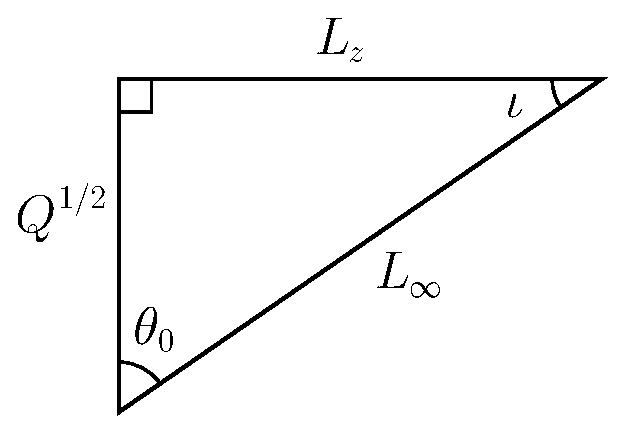
\includegraphics[width=0.35\textwidth]{./Images/Triangle.eps}
    \caption{The angular momenta $L_\infty$, $L_z$ and $\sqrt{Q}$ define a right-angled triangle. The acute angles are $\theta_0$, the extremal value of the polar angle, and $\iota$, the orbital inclination\cite{Glampedakis2002a}.}
   \label{fig:L_triangle}
\end{center}
\end{figure}
Let us now introduce a second angular variable\cite{Drasco2004}
\begin{equation}
\zeta = \zeta_0\cos^2\chi.
\end{equation}
Over one $2\pi$ period of $\chi$, $\theta$ oscillates over its full range, from its minimum value to its maximum and back. The geodesic equation for $\chi$ is
\begin{equation}
\rho^2\diff{\chi}{\tau} = \sqrt{Q + L_z^2},
\end{equation}
and may be integrated simply.

\section{Waveform Construction}

With the geodesic calculated for given angular momenta $L_z$ and $Q$, and initial starting positions, the orbiting body is assumed to follow this trajectory exactly: we ignore evolution due to the radiation of energy and angular momentum. From this we calculate the gravitational waveform using a semirelativistic approximation\cite{Ruffini1981}: we assume that the particle moves along a geodesic in the Kerr geometry, but radiates as if it were in flat spacetime. This quick-and-dirty technique is known as a numerical kludge (NK), and has been shown to approximate well results computed by more accurate methods\cite{Babak2007}.

\subsection{Kludge Approximation}

Numerical kludge approximations aim to encapsulate the main characteristics of a waveform by using the exact particle trajectory (ignoring inaccuracies from the evolution of the orbital parameters), whilst saving on computational time by using approximate waveform generation techniques. To start, we build an equivalent flat spacetime trajectory from the Kerr geodesic. This is done by identifying the Boyer-Lindquist coordinates with a set of flat-space coordinates; we consider two choices here:
\begin{enumerate}
\item Identify the Boyer-Lindquist coordinates with flat-space spherical polars \linebreak $\{r\sub{BL}, \theta\sub{BL}, \phi\sub{BL}\} \rightarrow \{r\sub{sph}, \theta\sub{sph}, \phi\sub{sph}\}$, then define flat-space Cartesian coordinates\cite{Gair2005, Babak2007}
\begin{equation}
\boldsymbol{x} = \left(r\sub{sph} \sin\theta\sub{sph}\cos\phi\sub{sph}, r\sub{sph} \sin\theta\sub{sph}\sin\phi\sub{sph}, r\sub{sph} \cos\theta\sub{sph}\right).
\end{equation}
\item Identify the Boyer-Lindquist coordinates with flat-space oblate-spheroidal coordinates $\{r\sub{BL}, \theta\sub{BL}, \phi\sub{BL}\} \rightarrow \{r\sub{ob}, \theta\sub{ob}, \phi\sub{ob}\}$ so that the flat-space Cartesian coordinates are
\begin{equation}
\boldsymbol{x} = \left(\sqrt{{r\sub{ob}}^2 + a^2} \sin\theta\sub{ob}\cos\phi\sub{ob}, \sqrt{{r\sub{ob}}^2 + a^2} \sin\theta\sub{ob}\sin\phi\sub{ob}, r\sub{ob} \cos\theta\sub{ob}\right).
\end{equation}
These are appealing because in the limit that $G \rightarrow 0$, so that the gravitating mass goes to zero, the Kerr metric in Boyer-Lindquist coordinates reduces to the Minkowski metric in oblate spheroidal coordinates.%\footnote{We must take the limit $G \rightarrow 0$, rather than $M_\bullet \rightarrow 0$ to avoid the problem of an over-extreme BH with $a > M_\bullet$.}
\end{enumerate}
In the limit of $a \rightarrow 0$, the two coincide, as they do in the limit of large $r\sub{BL}$. It must be stressed that there is no well motivated argument that either coordinate system must yield an accurate GW; their use is justified {\it post facto} by comparison with results obtained from more accurate, and computationally intensive, methods\cite{Gair2005, Babak2007}. This ambiguity in assigning flat-space coordinates reflects the inconsistency of the semi-relativistic approximation: the geodesic trajectory was calculated for the Kerr geometry; by moving to flat spacetime we lose the reason for its existence. However, this inconsistency should not be regarded as a major problem; it is just an artifact of the basic assumption that the shape of the trajectory is important for determining the character of the radiation, but the curvature of the spacetime in the vicinity of the source is not. By binding the particle to the exact geodesic, we ensure that the kludge waveform has spectral components at the correct frequencies, but by assuming flat spacetime for generation of GWs they will not have the correct amplitudes.

\subsection{Quadrupole-Octopole Formula}

Now we have a flat-space particle trajectory $x\sub{p}^\mu(\tau)$, we may apply a flat-space wave generation formula. We shall use the quadrupole-octopole formula to calculate the gravitational strain\cite{Press1977, Bekenstein1973}
\begin{equation}
h^{jk}(t, \boldsymbol{x}) = -\frac{2G}{c^6r}\left[\ddot{I}^{jk} - 2n_i\ddot{S}^{ijk} + n_i\dddot{M}^{ijk}\right]_{t'\, =\, t - cr}
\label{eq:Octopole}
\end{equation}
where an over-dot represents differentiation with respect to time $t$ (and not $\tau$), $t'$ is the retarded time, $r = \left|\boldsymbol{x} - \boldsymbol{x}\sub{p}\right|$ is the radial distance, $\boldsymbol{n}$ is the radial unit vector, and the mass quadrupole ${I}^{jk}$, current quadrupole ${S}^{ijk}$ and mass octopole ${M}^{ijk}$ are defined by
\begin{align}
{I}^{jk}(t') = {} & \intd{}{}{{x'}^j{x'}^kT^{00}(t', \boldsymbol{x'})}{^3x'}\\
{S}^{ijk}(t') = {} & \intd{}{}{{x'}^j{x'}^kT^{0i}(t', \boldsymbol{x'})}{^3x'}\\
{M}^{ijk}(t') = {} & \recip{c}\intd{}{}{{x'}^i{x'}^j{x'}^kT^{00}(t', \boldsymbol{x'})}{^3x'}.
\end{align}
This is correct for a slow moving source. It is the familiar quadrupole formula\cite{Misner1973, Hobson2006}, derived from linearized theory, but with the next order term included. For a point mass the energy-momentum tensor $T^{\mu\nu}$ contains a $\delta$-function which allows easy evaluation of the integrals of the various moments to give
\begin{align}
{I}^{jk} = {} & c^2\mu x\sub{p}^jx\sub{p}^k\\
{S}^{ijk} = {} & c\mu v\sub{p}^ix\sub{p}^jx\sub{p}^k\\
{M}^{ijk} = {} & c\mu x\sub{p}^ix\sub{p}^jx\sub{p}^k.
\end{align}
To evaluate \eqnref{Octopole} we need up to the third time derivative of the position. The velocity $\boldsymbol{v}\sub{p} = \dot{\boldsymbol{x}}\sub{p}$ can be calculated from the geodesic equations: dividing by $\linediff{t}{\tau}$ gives $\dot{r}$, $\dot{\theta}$ and $\dot{\phi}$ which can then be transformed to the Cartesian velocities assuming either the spherical or oblate spheroidal coordinate system.\footnote{There is again the problem of the sign of the geodesic equations; this is simply solved by taking the sign as calculated by finite differencing of the trajectory.} Expressions for the acceleration $\boldsymbol{a}\sub{p} = \ddot{\boldsymbol{x}}\sub{p}$ and the jerk $\boldsymbol{j}\sub{p} = \dddot{\boldsymbol{x}}\sub{p}$ are more involved, so these derivatives are found numerically using a simple difference formula to approximate the derivative as
\begin{equation}
\left.\diff{f}{t}\right|_{t_1} \approx \recip{2}\left[\frac{f(t_1) - f(t_0)}{t_1 - t_0} + \frac{f(t_2) - f(t_1)}{t_2 - t_1}\right],
\end{equation}
where $t_0$, $t_1$ and $t_2$ are subsequent (not necessarily uniformly spaced) time-steps.

Since we are only interested in GWs, we shall use the transverse-traceless (TT) gauge. The waveform is given in the TT gauge by\cite{Misner1973}
\begin{equation}
{h\super{TT}}_{jk} = P^l_jh_{lm}P^m_k - \recip{2}P_{jk}P^{lm}h_{lm},
\end{equation}
where the (spatial) projection operator $P_{ij}$ is
\begin{equation}
P_{ij} = \delta_{ij} - n_in_j.
\end{equation}

\section{Detection With LISA}

The LISA detector is a three-arm, spaceborne laser interferometer\cite{Bender1998, Danzmann2003}. The three arms form an equilateral triangle that rotates as the system's centre of mass follows a circular, heliocentric orbit, trailing $\ang{20}$ behind the Earth. To describe the detector configuration, and to transform from the MBH coordinate system to those of the detector, we will find it useful to define three coordinate systems: those of the BH at the galactic centre $x_\bullet^i$; ecliptic coordinates centred at the solar system barycentre $x_\odot^i$, and coordinates that co-rotate with the detector $x\sub{d}^i$. The MBH's coordinate system and the solar system coordinate system are depicted in \figref{BH_SS}.
\begin{figure}[tbhp]
\begin{center}
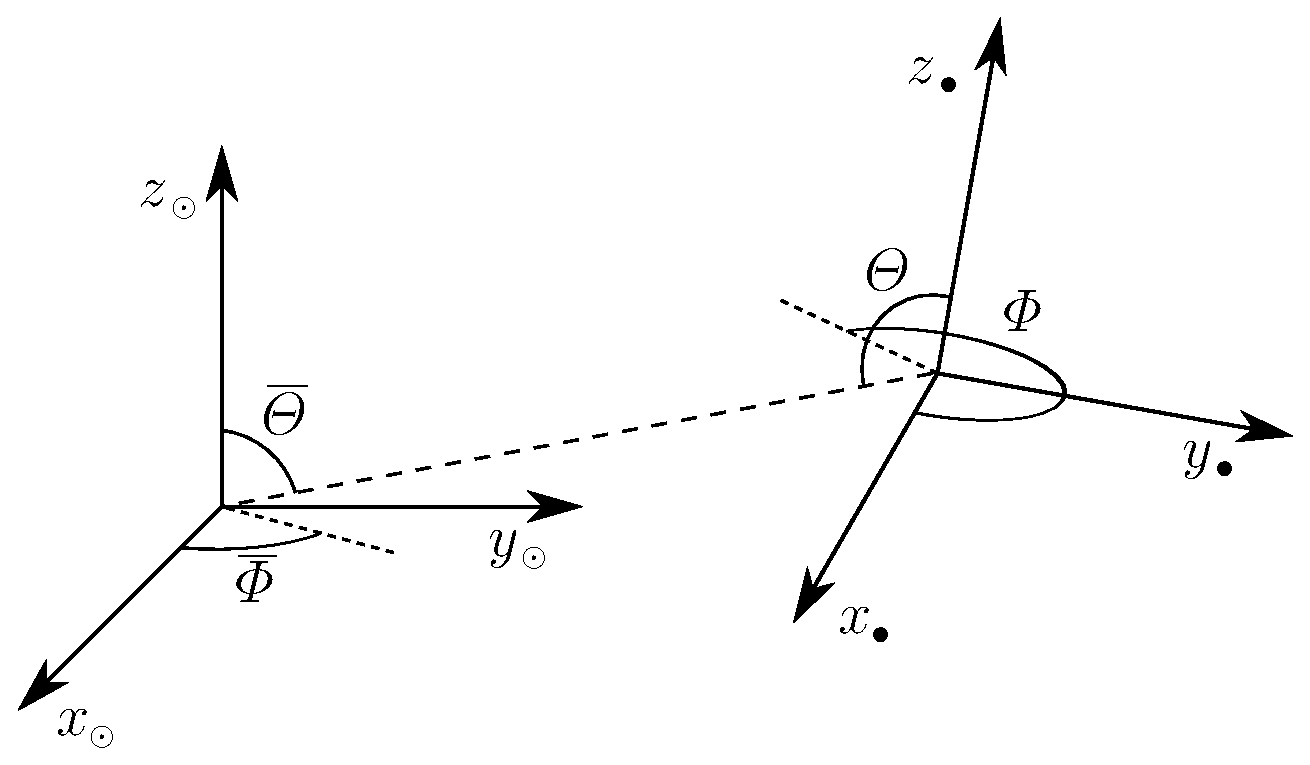
\includegraphics[width=0.65\textwidth]{./Images/BH_SS.eps}
    \caption{The relationship between the MBH's coordinate system $x_\bullet^i$ and the solar system coordinate system $x_\odot^i$. The MBH's spin axis is aligned with the $z_\bullet$-axis.}
   \label{fig:BH_SS}
\end{center}
\end{figure}
The currently envisioned LISA mission geometry is shown in \figref{SS_LISA}.
\begin{figure}[htbp]
\begin{center}
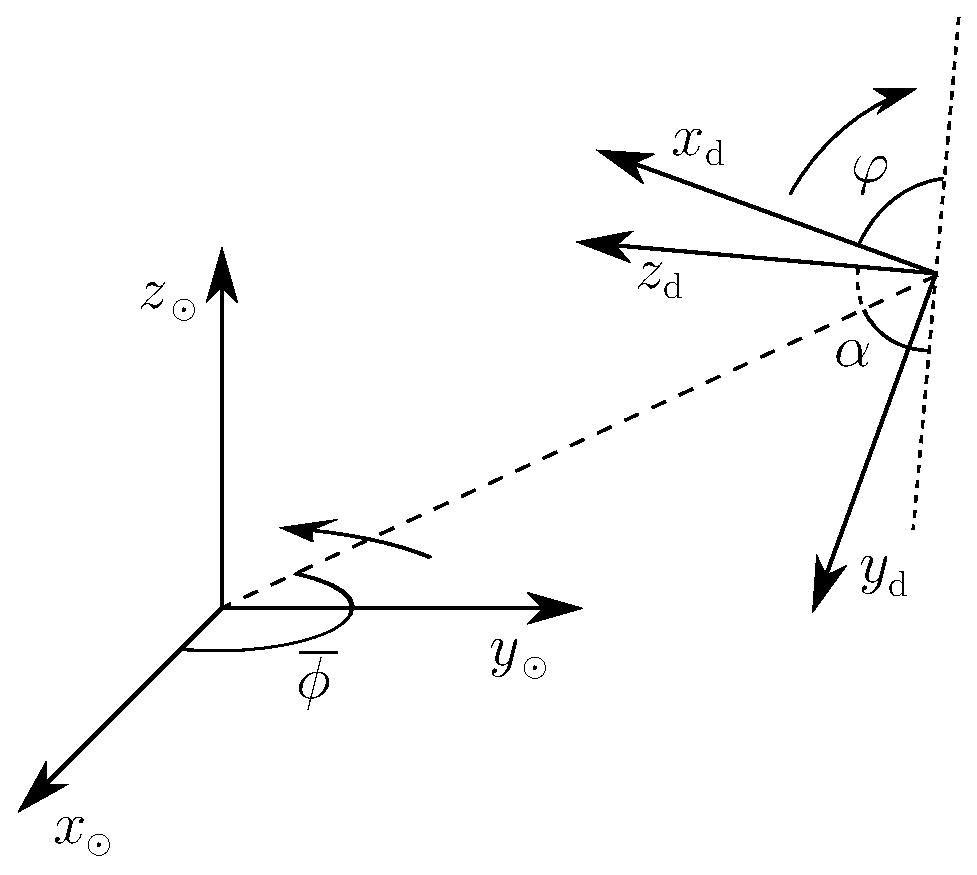
\includegraphics[width=0.5\textwidth]{./Images/SS_LISA.eps}
    \caption{The relationship between the detector coordinates $x\sub{d}^i$ and the ecliptic coordinates of the solar system $x_\odot^i$\cite{Bender1998}.}
   \label{fig:SS_LISA}
\end{center}
\end{figure}
We define the detector coordinates such that the detector-arms lie in the $x\sub{d}$-$y\sub{d}$ plane as shown in \figref{LISA_arms}.
\begin{figure}[htb]
\begin{center}
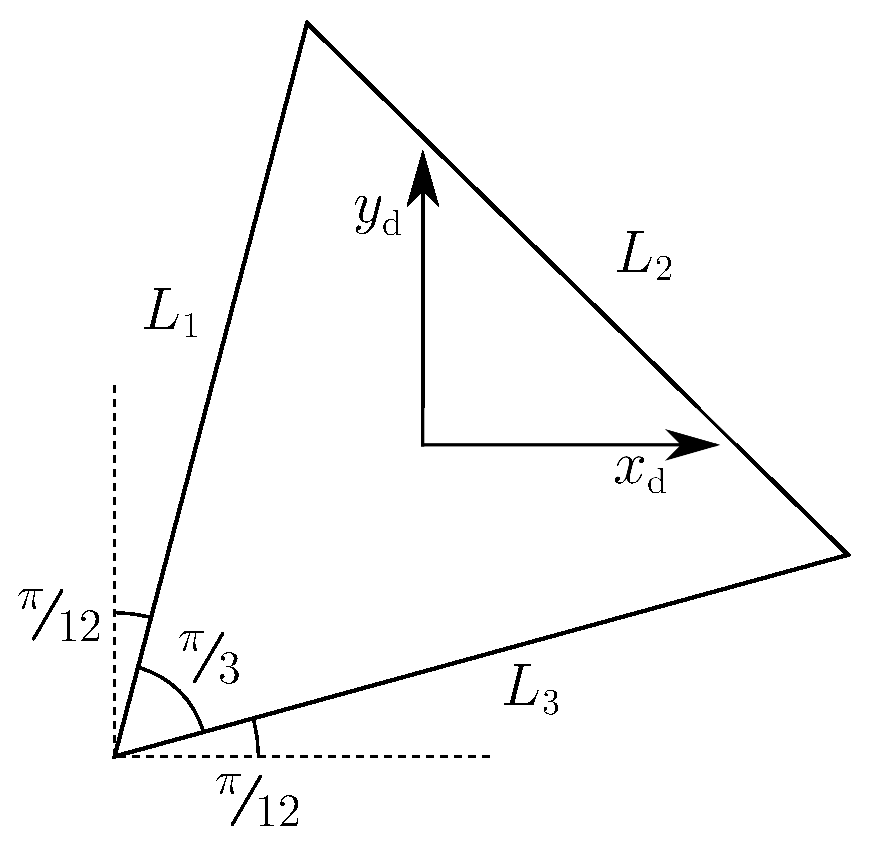
\includegraphics[width=0.35\textwidth]{./Images/LISA_arms.eps}
    \caption{The alignment of the three detector arms, with lengths $L_1$, $L_2$ and $L_3$, within the $x\sub{d}$-$y\sub{d}$ plane\cite{Cutler1998}. The origin of the detector coordinates coincides with the centre of mass of the constellation of satallites.}
   \label{fig:LISA_arms}
\end{center}
\end{figure}
The coordinate systems are related by a series of angles: $\Theta$ and $\Phi$ give the orientation of the solar system in the MBH's coordinates. These define the orientation of the MBH's spin axis $z_\bullet$. $\overline{\Theta}$ and $\overline{\Phi}$ give the position of the galactic centre in ecliptic coordinates. $\overline{\phi}$ gives LISA's orbital phase and $\varphi$ gives the rotational phase of the detector arms. Both of these vary linearly with time
\begin{equation}
\overline{\phi}(t) = \omega_\oplus t + \overline{\phi}_0; \quad \varphi(t) = -\omega_\oplus t + \varphi_0;
\end{equation}
where $\omega_\oplus$ corresponds to one rotation per year. Finally, $\alpha = \ang{60}$ is the inclination of the detector plane. We have computed the waveforms in the MBH's coordinates, however it is simplest to describe the measured signal using the detector's coordinates. To transform between coordinates we will use the matrix $A_{ij}$:
\begin{equation}
x\sub{d}^i = A^i_jx_\bullet^j; \quad h\sub{d}^{ij} = A^i_kA^j_lh_\bullet^{kl}.
\end{equation}
To define this, it is convenient to introduce angles
\begin{equation}
\Sigma = \overline{\Theta} + \Theta; \quad \delta = \overline{\phi} - \overline{\Phi}.
\end{equation}
The transformation matrix from the BH coordinates to the detector coordinates is
\begin{equation}
\left[A^i_j\right] = \begin{bmatrix}
a_{11} & a_{12} & a_{13} \\
a_{21} & a_{22} & a_{23} \\
a_{31} & a_{32} & a_{33}
\end{bmatrix};
\end{equation}
with elements
\begin{align}
a_{11} = {} & s_\varphi\left(c_\delta s_\Phi - s_\delta c_\Phi c_\Sigma\right) - c_\varphi \left[s_\alpha c_\Phi s_\Sigma - c_\alpha \left(c_\delta c_\Phi c_\Sigma + s_\delta s_\Sigma\right)\right]; \\
a_{12} = {} & -s_\varphi\left(c_\delta c_\Phi - s_\delta s_\Phi c_\Sigma\right) - c_\varphi \left[s_\alpha s_\Phi s_\Sigma - c_\alpha \left(c_\delta s_\Phi c_\Sigma + s_\delta s_\Sigma\right)\right]; \\
a_{13} = {} & s_\varphi s_\delta s_\Sigma - c_\varphi\left(s_\alpha c_\Sigma + c_\alpha c_\delta s_\Sigma\right); \\
a_{21} = {} & s_\varphi\left[s_\alpha c_\Phi s_\Sigma - c_\alpha \left(c_\delta c_\Phi c_\Sigma + s_\delta s_\Sigma\right)\right] - c_\varphi \left(c_\delta s_\Phi - s_\delta c_\Phi s_\Sigma\right); \\
a_{22} = {} & s_\varphi\left[s_\alpha s_\Phi s_\Sigma - c_\alpha \left(c_\delta s_\Phi c_\Sigma + s_\delta s_\Sigma\right)\right] - c_\varphi \left(c_\delta c_\Phi - s_\delta s_\Phi s_\Sigma\right); \\
a_{23} = {} & s_\varphi\left(s_\alpha c_\Sigma + c_\alpha c_\delta s_\Sigma\right) - c_\varphi s_\delta s_\Sigma; \\
a_{31} = {} & -s_\alpha\left(c_\delta c_\Phi c_\Sigma + s_\delta s_\Phi\right) - c_\alpha c_\Phi s_\Sigma; \\
a_{32} = {} & s_\alpha\left(s_\delta c_\Phi - c_\delta s_\Phi c_\Sigma\right) - c_\alpha s_\Phi s_\Sigma; \\
a_{33} = {} & s_\alpha c_\delta s_\Sigma - c_\alpha c_\Sigma;
\end{align}
where we define $s_\vartheta \equiv \sin \vartheta$ and $c_\vartheta \equiv \cos \vartheta$.

The strains measured in the three arms can be combined such that LISA behaves as a pair of $\ang{90}$ interferometers at $\ang{45}$ to each other (with signals scaled by $\nicefrac{\sqrt{3}}{2}$)\cite{Cutler1998}. We will denote the two detectors as I and II. If we label the change in the three arms lengths caused by GWs $\delta L_1$, $\delta L_2$ and $\delta L_3$, and use $L$ for the unperturbed length, then detector I measures strain
\begin{align}
h\sub{I}(t) = {} & \frac{\delta L_1 - \delta L_2}{L} \\
 = {} & \frac{\sqrt{3}}{2}\left(\recip{2} h\sub{d}^{xx} - \recip{2}h\sub{d}^{yy}\right),
\end{align}
and detector II measures
\begin{align}
h\sub{II}(t) = {} & \frac{\delta L_1 + \delta L_2 - 2 \delta L_3}{\sqrt{3}L} \\
 = {} & \frac{\sqrt{3}}{2}\left(\recip{2} h\sub{d}^{xy} + \recip{2} h\sub{d}^{yx}\right).
\end{align}
We will use vector notation $\boldsymbol{h}(t) = \left(h\sub{I}(t), h\sub{II}(t)\right) = \left\{h_A(t)\right\}$ to represent signals from both detectors.

The final consideration for calculating the signal measured by LISA is the time of arrival of the signal: LISA's orbital position changes with time. Fortunately over the timescales of interest for parabolic encounters, these changes are small. We will assume that the position of the solar system barycentre relative to the galactic centre is constant, at least over these short timescales: it is defined by the distance $R_0$ and the angles $\overline{\Theta}$ and $\overline{\Phi}$. The time of arrival at the solar system barycentre $t_\odot$ is then the appropriate retarded time. The time of detection $t\sub{d}$ to lowest order is then
\begin{equation}
t\sub{d} \simeq t_\odot - t\sub{AU}\cos\left[\overline{\phi}(t_\odot) - \overline{\Phi}\right]\sin\overline{\Theta},
\end{equation}
where $t\sub{AU}$ is the light travel-time for LISA's orbital radius. The time $t\sub{d}$ must be used for $\phi(t)$ and $\varphi(t)$.

\section{Signal Analysis}

\subsection{Frequency Domain Formalism}

At this stage we now know the GW $\boldsymbol{h}(t)$ that will be incident upon the LISA detector. We must now discuss how to analyse the waveform to extract the information it contains. We begin with a brief overview of the basic components of signal analysis used for GWs, with application to LISA in particular. This fixes the notation we will employ. A more complete discussion of material presented here can be found in the work of Finn\cite{Finn1992}, and Cutler and Flanagan\cite{Cutler1994}.

The actual measured strain $\boldsymbol{s}(t)$ will be the combination of the signal and the detector noise
\begin{equation}
\boldsymbol{s}(t) = \boldsymbol{h}(t) + \boldsymbol{n}(t),
\end{equation}
we will assume that the noise $n_A(t)$ is stationary and Gaussian. When analysing signals, it is most convenient to work with the Fourier transform
\begin{equation}
\tilde{g}(f) = \intd{-\infty}{\infty}{g(t)e^{2\pi i ft}}{t}.
\end{equation}
Since we have assumed Gaussianity for the noise signal $n_A(t)$, each Fourier component $\tilde{n}_A(f)$ also has a Gaussian probability distribution; the assumption of stationarity means that different Fourier components are uncorrelated, thus\cite{Cutler1994}
\begin{equation}
\left\langle\tilde{n}_A(f)\tilde{n}_B^*(f')\right\rangle_n = \recip{2}\delta(f - f')S_{AB}(f),
\end{equation}
where $\left\langle\ldots\right\rangle_n$ denotes the expectation value over the noise distribution, and $S_{AB}(f)$ is the (single-sided) noise spectral density. For simplicity, we may assume that the noise in the two detectors is uncorrelated, but share the same characterization so that\cite{Cutler1998}
\begin{equation}
S_{AB}(f) = S_n(f)\delta_{AB}.
\end{equation}
The functional form of the noise spectral density $S_n(f)$ for LISA is discussed below in \secref{Noise}.

The properties of the noise allow us to define a natural inner product and associated distance on the space of signals\cite{Cutler1994}
\begin{equation}
\innerprod{\boldsymbol{g}}{\boldsymbol{k}} = 2\intd{0}{\infty}{\frac{\tilde{g}_A^*(f)\tilde{k}_A(f) + \tilde{g}_A(f)\tilde{k}_A^*(f)}{S_n(f)}}{f}.
\label{eq:inner}
\end{equation}
Using this definition, the probability of a particular realization of noise $\boldsymbol{n}(t) = \boldsymbol{n}_0(t)$ is
\begin{equation}
p(\boldsymbol{n}(t) = \boldsymbol{n}_0(t)) \propto \exp\left[-\recip{2}\innerprod{\boldsymbol{n}_0}{\boldsymbol{n}_0}\right].
\end{equation}
Thus, if the incident waveform is given as $\boldsymbol{h}(t)$, the probability of measuring signal $\boldsymbol{s}(t)$ is
\begin{equation}
p(\boldsymbol{s}(t)|\boldsymbol{h}(t)) \propto \exp\left[-\recip{2}\innerprod{\boldsymbol{s}-\boldsymbol{h}}{\boldsymbol{s}-\boldsymbol{h}}\right].
\label{eq:sig_prob}
\end{equation}

\subsection{LISA Noise Curve}\label{sec:Noise}

LISA's noise has two sources: instrumental noise and confusion noise, primarily from white dwarf binaries. The latter may be divided into contributions from galactic and extragalactic binaries. In this work we use the noise model of Barack and Cutler\cite{Barack2004}. The shape of the noise curve can be seen in \figref{Noise}. The instrumental noise dominates at both high and low frequencies. The confusion noise is important at intermediate frequencies, and is responsible for the cusp around $f = \SI{1e-3}{\Hz}$.
\begin{figure}
\begin{center}
{\resizebox{0.65\textwidth}{!}{\import{./Images/}{Noise.tex}}}
\caption{Approximate noise curve for LISA\cite{Barack2004}. The solid line includes both instrumental and confusion noise, while the dashed line shows only instrumental.}
\label{fig:Noise}
\end{center}
\end{figure}

\subsection{Window Functions}

There is one remaining complication regarding signal analysis. When we perform a Fourier transform using a computer we must necessarily only transform a finite time-span (it is a discrete Fourier transform).\footnote{The time-span in this case is the length of time the trajectory was calculated for.} The effect of this is the same as transforming the true, infinite signal multiplied by a unit top hat function of width equal to the time-span. Fourier transforming this yields the true waveform convolved with a $\sinc$. If $\tilde{h}'(f)$ is the computed Fourier transform then
\begin{align}
\tilde{h}'(f) = {} & \intd{0}{\tau}{h(t)e^{2\pi i ft}}{t} \\
 = {} & \left[\tilde{h}(f) \ast e^{-\pi if\tau}\tau \sinc(\pi f\tau)\right],
\end{align}
where $\tilde{h}(f) = \mathscr{F}\{h(t)\}$, is the unwindowed Fourier transform. This windowing of the data is an inherent problem in the method; it will be as much of a problem when analysing signals from LISA as it is computing waveforms here. Windowing causes spectral leakage, which means that a contribution from large amplitude spectral components leaks into other components (sidelobes), obscuring and distorting the spectrum at these frequencies\cite{Jones1982,Harris1978}.

\Figref{Rectangular} shows the computed Fourier transforms for an example parabolic encounter.
\begin{figure}[htbp]
  \begin{center} \subfigure[]{\resizebox{0.45\textwidth}{!}{\import{./Images/}{h_I_Rectangular.tex}}} \quad
\subfigure[]{\resizebox{0.45\textwidth}{!}{\import{./Images/}{h_II_Rectangular.tex}}} \\
    \caption{Example spectra calculated using a rectangular window.  The high-frequency tail is the result of spectral leakage. The input parameters are: $M_\bullet = \num{4.3e6} M_\odot$, $a = 0.5 M_\bullet$, $\Theta = \pi/3$, $\Phi = 0$, $R_0 = \SI{8.33}{\kilo\parsec}$, $\overline{\Theta} = \ang{95.607669}$, $\overline{\Phi} = \ang{266.851760}$, $\overline{\phi}_0 = 0$, $\varphi_0 = 0$, $L_z = 10.44 M_\bullet$, $Q = 0.055 M_\bullet^2$, $\mu = 5 M_\odot$, $x_0 = \SI{3.5e12}{\metre}$, $y_0 = \SI{3.0e12}{\metre}$, $z_0 = \SI{1.0e11}{\metre}$; see \secref{Parameters} for a discussion of these parameters. The periapse distance is $r\sub{p} = 52.7 M_\bullet$. The high-frequency tail is the result of spectral leakage. The level of the LISA noise curve is indicated by the dashed line.}
    \label{fig:Rectangular}
  \end{center}
\end{figure}
The waveforms have two distinct regions: a low-frequency curve, and a high-frequency tail. The low-frequency signal is the spectrum we are interested in; the high-frequency components are the result of spectral leakage. The $\order{\nicerecip{f}}$ behaviour of the $\sinc$ gives the shape of the tail. This has possibly been misidentified by Burko and Khanna\cite{Burko2007} as the characteristic strain for parabolic encounters.

Despite being many orders of magnitude below the peak level, the high-frequency tail is still well above the noise curve for a wide range of frequencies. It will therefore contribute to the evaluation of any inner products, and may mask interesting features. Unfortunately this is a fundamental problem that cannot be resolved completely. However, it is possible to reduce the amount of spectral leakage using apodization: to improve the frequency response of a finite time series one can use a number of weighting window functions $w(t)$ which modify the impulse response in a prescribed way. The simplest window function is the rectangular (or Dirichlet) window; this is just the top hat described above. Other window functions are generally tapered. The introduction of a window function influences the spectrum in a manner dependent upon its precise shape; there are two distinct distortions: local smearing due to the finite width of the centre lobe, and distant leakage due to finite amplitude sidelobes. Choosing a window function is a trade-off between these two sources of error.

There is a wide range of window functions described in the literature\cite{Harris1978,Kaiser1980,Nuttall1981}. Since we are interested in a large dynamic range, it is necessary to pick a windowing function with exceptionally low sidelobes. We have opted for the Nuttall 4-term window with continuous first derivative\cite{Nuttall1981}.\footnote{The Blackman-Harris minimum 4-term window\cite{Harris1978, Nuttall1981}, and the Kaiser-Bessel window\cite{Harris1978, Kaiser1980} give almost identical results.} This has low peak sidelobe and asymptotically decays away as $\nicerecip{f^3}$. \Figref{Nuttall} shows the waveform obtained using this window.
\begin{figure}[htbp]
  \begin{center}
   \subfigure[]{\resizebox{0.45\textwidth}{!}{\import{./Images/}{h_I_Nuttall_first_derivative.tex}}} \quad
   \subfigure[]{\resizebox{0.45\textwidth}{!}{\import{./Images/}{h_II_Nuttall_first_derivative.tex}}} \\
    \caption{Example spectra calculated using Nuttall's 4-term window with continuous first derivative\cite{Nuttall1981}. The input parameters are identical to those used for \figref{Rectangular}. Although this window has good sidelobe behaviour, it is still not enough to suppress spectral leakage below the LISA noise level, the dashed line, at all frequencies.}
    \label{fig:Nuttall}
  \end{center}
\end{figure}
The spectral leakage is greatly reduced.

When using a tapered window function it is important to ensure that the window is centred upon the signal; otherwise the calculated transform will have a reduced amplitude.

\section{Parameter Estimation \& Waveforms}

\subsection{Model Parameters}\label{sec:Parameters}

The shape of the waveform depends on a number of parameters: those defining the MBH; those defining the companion object on its orbits, and those defining the LISA detector. Let us define $\boldsymbol{\lambda} = \{\lambda^1, \lambda^2, \ldots, \lambda^N\}$ as the set of $N$ parameters which define the GW. For our model the input parameters are:
\begin{enumerate}[leftmargin=*, widest=\:88--88.]%\setlength{\tabcolsep}{3pt}\begin{center}\begin{longtable}[0.85\textwidth]{r p{0.85\textwidth}}
\item[1.] The MBH's mass $M_\bullet$. This is currently well constrained by the observation of stellar orbits about Sgr A*\cite{Ghez2008, Gillessen2009}, with the best estimate being $M_\bullet = (4.31 \pm 0.36) \times 10^6 M_\odot$. However this depends upon the galactic centre distance $R_0$ being accurately known. If the uncertainty in this is included $M_\bullet = (3.95 \pm 0.06|\sub{stat} \pm 0.18|_{R_0, \, \mathrm{stat}} \pm  0.31|_{R_0, \, \mathrm{sys}}) \times 10^6 M_\odot (R_0 / \SI{8}{\kilo\parsec})^{2.19}$, where the errors are statistical independent of $R_0$, statistical from the determination of $R_0$, and systematic from $R_0$.
\item[2.] The spin parameter $a$. Naively we may expect this to be anywhere in the range $|a| < M_\bullet$, however the spin parameter may be limited by the accretion history. Considering the torque from radiation emitted by an accretion disc and swallowed by the BH it may be argued that $|a| \lesssim 0.998 M_\bullet$\cite{Thorne1974}. If the MBH grew via a series of randomly orientated accretion events, then the spin parameter can be low, and we would expect an average value $|a| \sim \numrange[tophrase=dash]{0.1}{0.3} M_\bullet$\cite{King2006, King2008}.
\item[3.] The polar angle $\Theta$ defining the propagation direction.
\item[4.] The solar system-galactic centre distance $R_0$. As for $M_\bullet$, this is constrained by stellar orbits, the best estimate being\cite{Gillessen2009} $R_0 = \SI[seperr]{8.33(35)}{\kilo\parsec}$.
\item[5, 6.] The coordinates of the MBH from the solar system barycentre $\overline{\Theta}$ and $\overline{\Phi}$. These may be taken as the coordinates of Sgr A*, as the radio source is expected to be within ten Schwarzscild radii of the MBH\cite{Reid2003}. At the epoch J2000.0\cite{Reid1999} $\overline{\Theta} = \ang{95.607669}$, $\overline{\Phi} = \ang{266.851760}$. This will change with time due to the rotation of the solar system about the galactic centre, the proper motion is about $\SI{6}{\milli\as\per\yr}$, mostly in the plane of the galaxy\cite{Reid1999, Backer1999, Reid2003}.
\item[7.] The angular momentum of the orbit about the MBH's spin axis $L_z$.
\item[8.] The Carter constant for the orbit $Q$.
\item[9.] The mass of the orbiting particle $\mu$. This will depend upon the type of object: whether it is a MS star, WD, NS or BH.
\item[10--12.] The initial position of the particle $(x_0, y_0, z_0)$. For specific values of $Q$ and $L_z$ there is a definite upper limit on $|z_0|/\sqrt{x_0^2+y_0^2}$ given by the size of $\theta_0$ from \eqnref{theta_0}.
\item[13, 14.] The orbital position of the LISA satellites given by $\overline{\phi}$ and $\varphi$.\\
\end{enumerate}%\end{longtable}\end{center}
The azimuthal angle $\Phi$ is omitted, since it arbitrarily defines the orientation of the MBH's $x$- and $y$-axes. We shall define it to be zero without loss of generality. We thus have a $14$-dimensional parameter space. However, for a given signal arrival time the orbital parameters of LISA will be known; we will not try to infer these. In lieu of anything better, we will assume fiducial initial values of zero, $\overline{\phi}_0 = 0$, $\varphi_0 = 0$.\footnote{The values of $\overline{\phi}_0$ and $\varphi_0$ do change the observed waveforms, altering the strain measured in the two arms. We do not investigate the full implications of this since we already have a large number of variables to consider, and because we will not know how $\overline{\phi}$ and $\varphi$ will be related until the mission geometry is finalised.} This leaves us with a $12$-dimensional parameter space to explore.

\subsection{Waveforms}

Figures \ref{fig:Orbit_1}--\ref{fig:Orbit_7} show example waveforms to demonstrate some of the possible variations in the signal. All these examples assume $M_\bullet = \SI{8.6e31}{\kg} \simeq \num{4.3e6} M_\odot$, $R_0 = \SI{8.33}{\kilo\parsec}$, $\overline{\Theta} = \ang{95.607669}$, $\overline{\Phi} = \ang{266.851760}$ and $\mu = \SI{1e31}{\kg} \simeq 5 M_\odot$; the other parameters are specified in the figure captions.
\begin{figure}[htbp]
  \begin{center}
   \subfigure[]{\resizebox{0.45\textwidth}{!}{\import{./Images/}{h_I_1.tex}}} \quad
   \subfigure[]{\resizebox{0.45\textwidth}{!}{\import{./Images/}{h_II_1.tex}}} \\
    \caption{Waveform for model parameters: $a = 0.5 M_\bullet$, $\Theta = \pi/3$, $L_z = 3.67 M_\bullet$, $Q = 0.409 M_\bullet^2$, $x_0 = \SI{3.0e12}{\metre}$, $y_0 = \SI{4.0e12}{\metre}$, $z_0 = \SI{2.0e11}{\metre}$. The periapse distance is $r\sub{p} = 4.67 M_\bullet$.}
    \label{fig:Orbit_1}
  \end{center}
\end{figure}
\begin{figure}[htbp]
  \begin{center}
   \subfigure[]{\resizebox{0.45\textwidth}{!}{\import{./Images/}{h_I_2.tex}}} \quad
   \subfigure[]{\resizebox{0.45\textwidth}{!}{\import{./Images/}{h_II_2.tex}}} \\
    \caption{Waveform for model parameters: $a = 0.5 M_\bullet$, $\Theta = \pi/3$, $L_z = 5.22 M_\bullet$, $Q = 0.055 M_\bullet^2$, , $x_0 = \SI{3.5e12}{\metre}$, $y_0 = \SI{3.5e12}{\metre}$, $z_0 = \SI{1.0e11}{\metre}$. The periapse distance is $r\sub{p} = 11.77 M_\bullet$.}
    \label{fig:Orbit_2}
  \end{center}
\end{figure}
\begin{figure}[htbp]
  \begin{center}
   \subfigure[]{\resizebox{0.45\textwidth}{!}{\import{./Images/}{h_I_5.tex}}} \quad
   \subfigure[]{\resizebox{0.45\textwidth}{!}{\import{./Images/}{h_II_5.tex}}} \\
    \caption{Waveform for model parameters: $a = 0.2 M_\bullet$, $\Theta = \pi/2$, $L_z = 10.45 M_\bullet$, $Q = 2.18 M_\bullet^2$, $x_0 = \SI{3.5e12}{\metre}$, $y_0 = \SI{3.5e12}{\metre}$, $z_0 = \SI{5.0e11}{\metre}$. The periapse distance is $r\sub{p} = 53.7 M_\bullet$.}
    \label{fig:Orbit_5}
  \end{center}
\end{figure}
\begin{figure}[htbp]
  \begin{center}
   \subfigure[]{\resizebox{0.45\textwidth}{!}{\import{./Images/}{h_I_6.tex}}} \quad
   \subfigure[]{\resizebox{0.45\textwidth}{!}{\import{./Images/}{h_II_6.tex}}} \\
    \caption{Waveform for model parameters: $a = 0.7 M_\bullet$, $\Theta = \pi/2$, $L_z = 5.22 M_\bullet$, $Q = 21.8 M_\bullet^2$, $x_0 = \SI{2.8e12}{\metre}$, $y_0 = \SI{2.8e12}{\metre}$, $z_0 = \SI{3.0e12}{\metre}$. The periapse distance is $r\sub{p} = 22.7 M_\bullet$.}
    \label{fig:Orbit_6}
  \end{center}
\end{figure}
\begin{figure}[htbp]
  \begin{center}
   \subfigure[]{\resizebox{0.45\textwidth}{!}{\import{./Images/}{h_I_7.tex}}} \quad
   \subfigure[]{\resizebox{0.45\textwidth}{!}{\import{./Images/}{h_II_7.tex}}} \\
    \caption{Waveform for model parameters: $a = 0.7 M_\bullet$, $\Theta = \pi/2$, $L_z = 15.7 M_\bullet$, $Q = 84.6 M_\bullet^2$, $x_0 = \SI{1.0e12}{\metre}$, $y_0 = \SI{4.2e12}{\metre}$, $z_0 = \SI{1.0e12}{\metre}$. The periapse distance is $r\sub{p} = 148 M_\bullet$.}
    \label{fig:Orbit_7}
  \end{center}
\end{figure}
The orbits specified in figures \ref{fig:Orbit_1}, \ref{fig:Orbit_2} and \ref{fig:Orbit_6} all loop once about the MBH --- they are the simplest zoom-whirl orbits. The others, including the orbit of \figref{Nuttall}, are simpler trajectories that are recognisable as parabolic in shape. There is a clear distinction between the two types of orbit, as the loops introduce higher frequency harmonics.

The waveforms plotted here all assume the oblate spheroidal coordinate system for the NK. Using spherical polars makes negligible difference: on the scale shown here the only discernible difference would be in the spikes of the high-frequency tail of the orbits with smaller periapses, and even that is minor. We therefore conclude that the choice of coordinates for the kludge approximation is unimportant, and shall continue with the oblate spheroidal coordinates for the rest of this work.

\subsection{Inference \& Fisher Matrices}

Having detected a GW signal $\boldsymbol{s}(t)$ we are interested in what we may learn about the source. We have an inference problem that may be solved by appropriate application of Bayes' Theorem\cite{Jaynes2003}: the probability distribution for our parameters given that we have detected the signal $\boldsymbol{s}(t)$ is given by the posterior
\begin{equation}
p(\boldsymbol{\lambda}|\boldsymbol{s}(t)) = \frac{p(\boldsymbol{s}(t)|\boldsymbol{\lambda})p(\boldsymbol{\lambda})}{p(\boldsymbol{s}(t))}.
\end{equation}
Here $p(\boldsymbol{s}(t)|\boldsymbol{\lambda})$ is the likelihood of the parameters, $p(\boldsymbol{\lambda})$ is the prior probability distribution for the parameters, and $p(\boldsymbol{s}(t)) = \intd{}{}{p(\boldsymbol{s}(t)|\boldsymbol{\lambda})}{^N \lambda}$ is, for our purposes, a normalising constant and may be ignored. The likelihood function depends upon the particular realization of noise. A particular set of parameters $\boldsymbol{\lambda}_0$ defines a waveform $\boldsymbol{h}_0(t) = \boldsymbol{h}(t; \boldsymbol{\lambda}_0)$, the probability that we observe signal $\boldsymbol{s}(t)$ for this GW is given by \eqnref{sig_prob}, so the likelihood is just
\begin{equation}
p(\boldsymbol{s}(t)|\boldsymbol{\lambda}_0) \propto \exp\left[-\recip{2}\innerprod{\boldsymbol{s}-\boldsymbol{h}_0}{\boldsymbol{s}-\boldsymbol{h}_0}\right].
\end{equation}
If we were to define this as a probability distribution for the parameters $\boldsymbol{\lambda}$, then the modal values would be the maximum-likelihood parameters $\boldsymbol{\lambda}\sub{ML}$. The waveform $h(t; \boldsymbol{\lambda}\sub{ML})$ would be the signal closest to $\boldsymbol{s}(t)$ in the space of all signals, where distance is defined using the inner product \eqnref{inner}\cite{Cutler1994}.

In the limit of a high signal-to-noise ratio (SNR), we may approximate this as\cite{Vallisneri2008}
\begin{equation}
p(\boldsymbol{s}(t)|\boldsymbol{\lambda}_0) \propto \exp\left[-\recip{2}\innerprod{\partial_a\boldsymbol{h}}{\partial_b\boldsymbol{h}}\left(\lambda^a - \langle\lambda^a\rangle_\ell\right)\left(\lambda^b - \langle\lambda^b\rangle_\ell\right)\right],
\end{equation}
where the mean is defined as
\begin{equation}
\langle\lambda^a\rangle_\ell = \frac{\intd{}{}{\lambda^a p(\boldsymbol{s}(t)|\boldsymbol{\lambda})}{^N \lambda}}{\intd{}{}{p(\boldsymbol{s}(t)|\boldsymbol{\lambda})}{^N \lambda}}.
\end{equation}
Using the high SNR limit approximation, this mean is just the maximum-likelihood value $\langle\lambda^a\rangle_\ell = \lambda^a\sub{ML}$. The quantity
\begin{equation}
\Gamma_{ab} = \innerprod{\partial_a\boldsymbol{h}}{\partial_b\boldsymbol{h}}
\end{equation}
is the Fisher information matrix. We see that it controls the variance of the likelihood distribution.

The form of the posterior distribution will depend upon the nature of the prior information. If we have an uninformative prior, such that $p(\boldsymbol{\lambda})$ is a constant, then the posterior distribution would be determined by the likelihood. In the high SNR limit, we would obtain a Gaussian with variance-covariance matrix
\begin{equation}
\boldsymbol{\Sigma} = \boldsymbol{\Gamma}^{-1}.
\end{equation}
The Fisher information matrix gives the uncertainty associated with the estimated parameter values, in this case the maximum-likelihood values. If the prior were to restrict the allowed range for a parameter, for example, as is the case for the spin parameter $a$, then the posterior would be a truncated Gaussian, and $\boldsymbol{\Gamma}^{-1}$ would no longer represent the variance-covariance. If the prior was approximately Gaussian with variance-covariance matrix $\boldsymbol{\Sigma}_0$, then the posterior would also be Gaussian.\footnote{If we only know the typical value and spread of a parameter then a Gaussian is the maximum entropy prior\cite{Jaynes2003}: the prior that is least informative given what we do know, the prior that best reflects our state of ignorance.} The posterior variance-covariance would be\cite{Cutler1994, Vallisneri2008}
\begin{equation}
\boldsymbol{\Sigma} = \left(\boldsymbol{\Gamma} + \boldsymbol{\Sigma}_0^{-1}\right)^{-1}.
\end{equation}
From this the inverse Fisher matrix $\boldsymbol{\Gamma}^{-1}$ is an upper bound on the size of the posterior covariance matrix.\footnote{It may also be shown to be the Cram\'{e}r-Rao bound on the error covariance of an unbiased estimator\cite{Cutler1994, Vallisneri2008}. Thus it represents the frequentist error: the lower bound on the covariance for an unbiased parameter estimator $\boldsymbol{\lambda}\sub{est}$ calculated from an infinite set of experiments with the same signal $\boldsymbol{h}(t)$ but different realizations of the noise $\boldsymbol{n}(t)$.}

As a first estimate of what we may learn from parabolic encounters we have only looked at the Fisher information matrix elements. If these are large then we expect we would be able to precisely determine a parameter, whereas if they are small we would not be able to learn much more than we already believe from our prior knowledge.

\subsection{Inverse Fisher Matrices}

Calculating the inverse Fisher matrix for example orbits, we find that there is a large degeneracy between the mass $\mu$ and the distance $R_0$. This is not surprising since the primary role of both is determining the amplitude of the waveform in \eqnref{Octopole}. This is the only place that $\mu$ appears. We will not be able to determine both from an extreme mass-ratio burst (EMRB), unless we can determine the mass of the object by other means, which seems unlikely. It appears that we must give up on determining $R_0$. Instead we should accept our prior value and remove $R_0$ from our parameter set.

The inverse Fisher matrix's elements for some example orbits are tabulated in the appendix. For the values presented here the parameters are normalised with respect to their maximum likelihood values $\widehat{\lambda}^a = \lambda^a/\lambda\sub{ML}^a$; the Fisher matrices are calculated by differentiating with respect to these parameters so that $\boldsymbol{\Gamma}^{-1}$ gives the relative variance-covariance.

There are a few general properties. The parameters $M_\bullet$ and $\Theta$ always have relatively small variances. These parameters are crucial for defining the BH system: $M_\bullet$ sets the scale for the system and $\Theta$ the orientation. Note that if $a$ were small, the spacetime would be almost spherically symmetric and we would expect a large variance for $\Theta$. The angular momentum $L_z$ also has a small variance, it is important for specifying the orbit; its partner $Q$, however, does not always have a small variance, in fact in some cases it has one of the largest. This appears to correlate with the size of the covariance of $Q$: the orbits with the smallest periapses have relatively large covariances for the set of parameters $a$, $Q$ and $z_0$, indicating that there is some degeneracy between these. In these cases $Q$ has a much larger variance, as does $z_0$. The initial coordinates $x_0$, $y_0$ and $z_0$ typically have small variance, the exception being the aforementioned case for $z_0$.

The parameters with the largest variances are $\overline{\Theta}$ and $\mu$. The large variance of $\Theta$ reflects the poor angular resolution of gravitational wave detectors; $\overline{\Phi}$ has a smaller variance as a change in azimuthal position changes the spectra observed in the two detector arms. The particle mass $\mu$ has a large variance since it only alters the amplitude of the spectrum and not its shape.

From this preliminary look at a few example orbits, it appears that we should be able to infer the mass of the Kerr BH at the galactic centre from an EMRB. We can gain information regarding the spin of the MBH if the orbit's periapsis is sufficiently small --- we could learn nothing from the orbit of \tabref{Fisher_7}. The Fisher matrix analysis suggests that we should be able to accurately infer the spin orientation; however it seems likely that there could be difficulties for small spin values. This will require further investigation. It seems unlikely that we will be able to improve upon our current best estimate for the position of the MBH, but this is already well constrained. What is particularly exciting is the amount of information we could obtain from a single encounter, which may be all that we would have the opportunity to observe with LISA. Taking the results of \tabref{Fisher_3}, which are for an orbit of periapsis $r\sub{p} = 52.7 M_\bullet$, as an example, we could infer maximum-likelihood values $M_\bullet = (4.32 \pm 0.07) \times 10^6 M_\odot$, $a = (0.50 \pm 0.02) M_\bullet$, and $\Theta = {(60.0 \pm 1.6)\degree}$. Here we have ignored uncertainty introduced by the error in $R_0$, but we have also not considered additional information from our prior knowledge. While further work will be needed to be certain how much we could expect to learn from EMRBs, this is encouraging.

\section{Energy Spectra}

To check that the NK waveforms are sensible, we may compare the energy spectra calculated from these waveforms with those obtained from the classic treatment of Peters and Matthews\cite{Peters1963, Peters1964}. This calculates GW emission for Keplerian orbits in flat spacetime, assuming only quadrupole radiation. The spectrum produced should be similar to that obtained from the NK in weak fields, that is for orbits with a large periapsis; however we do not expect an exact match because of the differing input physics and various approximations.  We do not intend to use the kludge waveforms to calculate an accurate energy flux: this would be inconsistent as we assume that the orbits do not evolve with time. We only calculate the energy flux as a sanity check; to check that the kludge approximation is consistent with other approaches.

\subsection{Kludge Spectrum}

Our gravitational wave in the TT gauge has momentum pseudotensor\cite{Misner1973}
\begin{equation}
T_{\mu\nu} = \frac{c^4}{32\pi G}\left\langle\partial_\mu h_{ij} \partial_\nu h^{ij}\right\rangle,
\end{equation}
where $\langle\ldots\rangle$ indicates averaging over several wavelengths, or equivalently averaging over several periods. Thus, the flux of energy through a sphere of radius $r = R$ is
\begin{equation}
\diff{E}{t} = \frac{c^3}{32\pi G} R^2 \int{\dd\Omega}\left\langle\diff{h_{ij}}{t}\diff{h^{ij}}{t}\right\rangle,
\end{equation}
with $\int{\dd\Omega}$ representing integration over all solid angles. From \eqnref{Octopole} we see that the waves have a $\nicerecip{r}$ dependence, so if we define
\begin{equation}
h_{ij} = \frac{H_{ij}}{r},
\end{equation}
we see that the flux is independent of $R$, as required for energy conservation,
\begin{equation}
\diff{E}{t} = \frac{c^3}{32\pi G} \int{\dd\Omega}\left\langle\diff{H_{ij}}{t}\diff{H^{ij}}{t}\right\rangle.
\end{equation}
If we now integrate to find the total energy emitted we obtain
\begin{equation}
E = \frac{c^3}{32\pi G} \int{\dd\Omega}\int_{-\infty}^{\infty}{\dd t} \, \diff{H_{ij}}{t}\diff{H^{ij}}{t}.
\end{equation}
Since we are considering all time, the localization of the energy is no longer of importance and so it is unnecessary to average over several periods. If we switch to Fourier representation $\widetilde{H}_{ij}(f) = \mathscr{F}\{H_{ij}(t)\}$, then
\begin{align}
E = {} & \frac{c^3}{32\pi G} \int{\dd\Omega}\int_{-\infty}^{\infty}{\dd t}\intd{-\infty}{\infty}{}{f} \, 2\pi i f \widetilde{H}_{ij}(f)e^{2\pi i f t}\int_{-\infty}^{\infty}{\dd f'} \, 2\pi i f' \widetilde{H}^{ij}(f')e^{2\pi i f' t} \nonumber \\
 = {} & \frac{\pi c^3}{8 G} \int{\dd\Omega}\int_{-\infty}^{\infty}{\dd f} \, f^2 \widetilde{H}_{ij}(f)\widetilde{H}^{ij}(-f) \nonumber \\
 = {} & \frac{\pi c^3}{4 G} \int{\dd\Omega}\int_{0}^{\infty}{\dd f} \, f^2 \widetilde{H}^{ij}(f)\widetilde{H}_{ij}^*(f).
\end{align}
Here we have used the fact that the signal is real so that $\widetilde{H}_{ij}^*(f) = \widetilde{H}_{ij}(-f)$. Using this we can identify the energy spectrum as
\begin{align}
\diff{E}{f} = \frac{\pi c^3}{4 G} \intd{}{}{}{\Omega} \, f^2 \widetilde{H}^{ij}(f)\widetilde{H}_{ij}^*(f).
\label{eq:NK_dEdf}
\end{align}

\subsection{Peters \& Matthews Spectrum}

To calculate the energy spectrum for a parabolic orbit, we follow the derivation of Gair\cite{Gair2010}. Peters and Matthews give the power radiated into the $n$th harmonic of the orbital angular frequency as
\begin{equation}
P(n) = \frac{32}{5}\frac{G^4}{c^5}\frac{M_\bullet^2\mu^2(M_\bullet + \mu)(1-e)^5}{{r\sub{p}}^5}g(n,e)
\label{eq:PM_P}
\end{equation}
where the function $g(n,e)$ is defined in terms of Bessel functions of the first kind
\begin{align}
g(n,e) = {} & \frac{n^4}{32}\left\{\left[J_{n-2}(ne) - 2eJ_{n-1}(ne) + \frac{2}{n}J_n(ne) + 2eJ_{n+1}(ne) - J_{n+2}(ne)\right]^2 \right. \nonumber \\
 & + \left. \left(1 - e^2\right)\left[J_{n-2}(ne) - 2J_n(ne) + J_{n+2}(ne)\right]^2 + \frac{4}{3n^2}\left[J_n(ne)\right]^2\right\}.
\end{align}
The Keplerian orbital frequency is
\begin{align}
{\omega_0}^2 = {} & \frac{G(M_\bullet + \mu)(1-e)^3}{{r\sub{p}}^3}\\
 = {} & (1-e)^3{\omega\sub{c}}^2,
\label{eq:Kepler_freq}
\end{align}
where $\omega\sub{c}$ is defined as the orbital angular frequency of a circular orbit of radius equal to $r\sub{p}$. The total energy radiated into the $n$th harmonic, that is at frequency $\omega_n = n\omega_0$, is the power multiplied by the orbital period
\begin{equation}
E(n) = \frac{2\pi}{\omega_0}P(n);
\label{eq:E(n)}
\end{equation}
as $e \rightarrow 1$ for a parabolic orbit, $\omega_0 \rightarrow 0$ so the orbital period becomes infinite. We may therefore identify the energy radiated per orbit with the total orbital energy radiated. Since the spacing of harmonics is $\Delta\omega = \omega_0$, we may identify the energy spectrum
\begin{equation}
\left.\diff{E}{\omega}\right|_{\omega_n}\omega_0 = E(n).
\end{equation}
Using the above relations, and changing to linear frequency $2\pi f = \omega$, we obtain
\begin{align}
\left.\diff{E}{f}\right|_{f_n} = {} & \frac{128\pi^2}{5}\frac{G^3}{c^5}\frac{M_\bullet^2\mu^2}{r\sub{p}^2}(1-e)^2g(n,e) \\
 = {} & \frac{4\pi^2}{5}\frac{G^3}{c^5}\frac{M_\bullet^2\mu^2}{r\sub{p}^2}\ell(n,e),
\label{eq:PM_spectrum}
\end{align}
where we have defined the function $\ell(n,e)$ in the last line. For a parabolic orbit, we now have to take the limit of $\ell(n,e)$ as $e \rightarrow 1$. For this we shall use a number of properties of Bessel functions, and will make frequent reference to Watson\cite{Watson1995}.

We shall simplify $\ell(n,e)$ using the recurrence formulae (Watson\cite{Watson1995} 2.12)
\begin{align}
J_{\nu-1}(z) + J_{\nu+1}(z) = {} & \frac{2\nu}{z}J_\nu(z)\\
J_{\nu-1}(z) - J_{\nu+1}(z) = {} & 2J'_\nu(z).
\end{align}
We shall also eliminate $n$ using
\begin{align}
n = {} & \frac{\omega_n}{\omega_0} \nonumber \\
= {} & (1-e)^{-3/2}\widetilde{f}.
\end{align}
where $\widetilde{f} = \omega_n/\omega\sub{c} = f_n/f\sub{c}$ is a dimensionless frequency. We begin by breaking $\ell$ into three parts
\begin{align}
\ell = {} & \underbrace{(1-e)^2n^4\left[J_{n-2} - 2eJ_{n-1} + \frac{2}{n}J_n + 2eJ_{n+1} - J_{n+2}\right]^2}_{\ell_1} \nonumber \\
  & + \underbrace{(1-e)^3(1+e)n^4\left[J_{n-2} - 2J_n + J_{n+2}\right]^2}_{\ell_2} + \underbrace{\frac{4(1-e)^2n^2}{3}\left[J_n\right]^2}_{\ell_3}.
\end{align}
We have suppressed the argument of the Bessel functions for brevity. Tackling each term of $\ell$ in turn we obtain
\begin{align}
\ell_1(\widetilde{f},e) = {} & \left[\frac{4(1+e)\widetilde{f}^2}{e}\frac{J'_n}{1-e} + 2\frac{e-2}{e}\widetilde{f}\frac{J_n}{(1-e)^{1/2}}\right]^2\\
\ell_2(\widetilde{f},e) = {} & 16(1+e)\left[\frac{(1+e)\widetilde{f}^2}{e^2}\frac{J_n}{(1-e)^{1/2}} - \widetilde{f}\frac{J'_n}{e}\right]^2\\
\ell_3(\widetilde{f},e) = {} & \frac{4\widetilde{f}^2}{3}\left[{J_n}{(1-e)^{1/2}}\right]^2.
\end{align}
To take the limit of these we need to find the limiting behaviour of Bessel functions. We shall define two new functions
\begin{equation}
A(\widetilde{f}) = \lim_{e\rightarrow 1}\left\{\frac{J_n}{(1-e)^{1/2}}\right\}; \quad B(\widetilde{f}) = \lim_{e\rightarrow 1}\left\{\frac{J'_n}{1-e}\right\}.
\end{equation}
To give a well defined energy spectrum, both of these must be finite. In this case we see that the second term in $\ell_2$ should go to zero.

The Bessel function has an integral representation
\begin{equation}
J_\nu(z) = \recip{\pi}\intd{0}{\pi}{\cos(\nu\theta - z\sin\theta)}{\theta},
\end{equation}
we want the limit of this for $\nu \rightarrow \infty$, $z \rightarrow \infty$, with $z \leq \nu$. We will use the stationary phase approximation to argue that the predominant contribution to the integral comes from when the argument of the cosine is approximately zero, that is for small $\theta$ (Watson\cite{Watson1995} 8.2, 8.43). In this case we have
\begin{align}
J_\nu(z) \sim {} & \recip{\pi}\intd{0}{\pi}{\cos\left(\nu\theta - z\theta + \frac{z}{6}\theta^3\right)}{\theta}\\
 \sim {} & \recip{\pi}\intd{0}{\infty}{\cos\left(\nu\theta - z\theta + \frac{z}{6}\theta^3\right)}{\theta};
\end{align}
this last expression is an Airy integral. The Airy integral has a standard form (Watson\cite{Watson1995} 6.4)
\begin{equation}
\intd{0}{\infty}{\cos(t^3 + xt)}{t} = \frac{\sqrt{x}}{3}K_{1/3}\left(\frac{2x^{3/2}}{3^{3/2}}\right),
\end{equation}
where $K_\nu(z)$ is a modified Bessel function of the second kind. Using this to evaluate our limit gives
\begin{equation}
J_\nu(z) \sim \recip{\pi}\sqrt{\frac{2(\nu - z)}{3z}}K_{1/3}\left(\frac{2^{3/2}}{3}\sqrt{\frac{(\nu -z)^3}{z}}\right).
\end{equation}
For our particular case we have
\begin{equation}
\nu = (1 - e)^{-3/2}\widetilde{f}; \quad z = (1 - e)^{-3/2}e\widetilde{f};
\end{equation}
\begin{equation}
\frac{\nu - z}{z} = (1 - e); \quad \frac{(\nu - z)^3}{z} = \widetilde{f}^2;
\end{equation}
so we find
\begin{equation}
J_n(ne) \sim \recip{\pi}\sqrt{\frac{2}{3}}(1-e)^{1/2}K_{1/3}\left(\frac{2^{3/2}\widetilde{f}}{3}\right),
\end{equation}
thus
\begin{equation}
A(\widetilde{f}) = \recip{\pi}\sqrt{\frac{2}{3}}K_{1/3}\left(\frac{2^{3/2}\widetilde{f}}{3}\right)
\end{equation}
is well defined.

Now finding the derivative
\begin{align}
J'_\nu(z) = {} & \recip{2}\left[J_{\nu-1}(z) - J_{\nu+1}(z)\right] \nonumber \\
 \sim {} & \recip{2\pi}\left[\sqrt{\frac{2(\nu -1 - z)}{3z}}K_{1/3}\left(\frac{2^{3/2}}{3}\sqrt{\frac{(\nu - 1 - z)^3}{z}}\right) \right. \nonumber \\
  & \left. - \sqrt{\frac{2(\nu +1 - z)}{3z}}K_{1/3}\left(\frac{2^{3/2}}{3}\sqrt{\frac{(\nu + 1 - z)^3}{z}}\right)\right].
\end{align}
For our case
\begin{align}
\sqrt{\frac{\nu \pm 1 - z}{z}} = {} & (1 - e)^{1/2}\left[1 \pm \frac{(1-e)^{1/2}}{2\widetilde{f}} + \ldots \, \right];\\
\sqrt{\frac{(\nu \pm 1 - z)^{3/2}}{z}} = {} & \widetilde{f}\left[1 \pm \frac{3(1-e)^{1/2}}{2\widetilde{f}} + \ldots \, \right];
\end{align}
and so
\begin{align}
J'_n(ne) \sim {} & \recip{2\pi}\sqrt{\frac{2}{3}}(1-e)^{1/2}\left\{\left[1 - \frac{(1-e)^{1/2}}{2\widetilde{f}}\right]K_{1/3}\left(\frac{2^{3/2}\widetilde{f}}{3}\left[1 - \frac{3(1-e)^{1/2}}{2\widetilde{f}}\right]\right) \right. \nonumber \\
 & \left. - \left[1 + \frac{(1-e)^{1/2}}{2\widetilde{f}}\right]K_{1/3}\left(\frac{2^{3/2}\widetilde{f}}{3}\left[1 - \frac{3(1-e)^{1/2}}{2\widetilde{f}}\right]\right)\right\}\nonumber \\
 \sim {} & \frac{-1}{2\pi}\sqrt{\frac{2}{3}}(1-e)\left[2^{3/2}K'_{1/3}\left(\frac{2^{3/2}\widetilde{f}}{3}\right) + \recip{\widetilde{f}}K_{1/3}\left(\frac{2^{3/2}\widetilde{f}}{3}\right)\right].
\end{align}
We may re-express the derivative using the recurrence formula (Watson\cite{Watson1995} 3.71)
\begin{equation}
K_{\nu-1}(z) - K_{\nu+1}(z) = -2K'_\nu(z)
\end{equation}
to give
\begin{equation}
J'_n(ne) \sim \frac{1-e}{\sqrt{3}\pi}\left[K_{-2/3}\left(\frac{2^{3/2}\widetilde{f}}{3}\right) + K_{4/3}\left(\frac{2^{3/2}\widetilde{f}}{3}\right) - \recip{\sqrt{2}\widetilde{f}}K_{1/3}\left(\frac{2^{3/2}\widetilde{f}}{3}\right)\right].
\end{equation}
And so finally,
\begin{equation}
B(\widetilde{f}) = \recip{\sqrt{3}\pi}\left[K_{-2/3}\left(\frac{2^{3/2}\widetilde{f}}{3}\right) + K_{4/3}\left(\frac{2^{3/2}\widetilde{f}}{3}\right) - \recip{\sqrt{2}\widetilde{f}}K_{1/3}\left(\frac{2^{3/2}\widetilde{f}}{3}\right)\right],
\end{equation}
which is also well defined.

Having obtained expressions for $A(\widetilde{f})$ and $B(\widetilde{f})$ in terms of standard functions, we may now calculate the energy spectrum for a parabolic orbit. From \eqnref{PM_spectrum} we have
\begin{equation}
\diff{E}{f} = \frac{4\pi^2}{5}\frac{G^3}{c^5}\frac{M_\bullet^2\mu^2}{r\sub{p}^2}\ell\left(\frac{f}{f\sub{c}}\right),
\label{eq:PM_dEdf}
\end{equation}
where we have used the limit
\begin{align}
\ell(\widetilde{f}) = {} & \lim_{e \rightarrow 1}\left\{\ell(n,e)\right\} \nonumber \\
 = {} & \left[8\widetilde{f}B(\widetilde{f}) - 2\widetilde{f}A(\widetilde{f})\right]^2 + \left(128\widetilde{f}^4 + \frac{4\widetilde{f}^2}{3}\right)\left[A(\widetilde{f})\right]^2.
\end{align}

To check the validity of this limit we may calculate the total energy radiated. We should be able to calculate this by integrating \eqnref{PM_dEdf} over all frequencies, or alternatively by summing the energy radiated into each harmonic. For consistency, the two approaches should yield the same result. First, summing over harmonics we obtain
\begin{align}
E\sub{sum} = {} & \sum_n E(n) \nonumber \\
 = {} & \frac{64\pi}{5}\frac{G^3}{c^5}\frac{M_\bullet^2\mu^2}{r\sub{p}^2}\omega\sub{c}(1-e)^{7/2}\sum_n g(n,e),
\end{align}
where we have used equations \eqref{eq:PM_P}, \eqref{eq:Kepler_freq} and \eqref{eq:E(n)}. Peters and Matthews\cite{Peters1963} provide the result
\begin{equation}
\sum_n g(n,e) = \frac{1 + \nicefrac{73}{24}\, e^2 + \nicefrac{37}{96}\, e^4}{(1-e^2)^{7/2}}.
\end{equation}
Using this,
\begin{equation}
E\sub{sum} = \frac{64\pi}{5}\frac{G^3}{c^5}\frac{M_\bullet^2\mu^2}{r\sub{p}^2}\omega\sub{c}\frac{1 + \nicefrac{73}{24}\, e^2 + \nicefrac{37}{96}\, e^4}{(1+e^2)^{7/2}}.
\end{equation}
This is perfectly well behaved as $e \rightarrow 1$. Taking the limit for a parabolic orbit, the total energy radiated is
\begin{equation}
E\sub{sum} = \frac{85\pi}{2^{5/2}3}\frac{G^3}{c^5}\frac{M_\bullet^2\mu^2}{r\sub{p}^2}\omega\sub{c}.
\end{equation}
Integrating over the energy spectrum, \eqnref{PM_dEdf}, gives
\begin{align}
E\sub{int} = {} & \intd{0}{\infty}{\diff{E}{f}}{f} \nonumber \\
 = {} & \frac{2\pi}{5}\frac{G^3}{c^5}\frac{M_\bullet^2\mu^2}{r\sub{p}^2}\omega\sub{c}\intd{0}{\infty}{\ell(\widetilde{f})}{\widetilde{f}}.
\end{align}
The integral can be easily evaluated numerically showing
\begin{align}
\intd{0}{\infty}{\ell(\widetilde{f})}{\widetilde{f}} = {} & 12.5216858\ldots \nonumber \\
 = {} & \frac{425}{2^{7/2}3},
\end{align}
and so we find that the two total energies are consistent
\begin{align}
\label{eq:PM_total}
E\sub{int} = {} & \frac{85\pi}{2^{5/2}3}\frac{G^3}{c^5}\frac{M_\bullet^2\mu^2}{r\sub{p}^2}\omega\sub{c} \\
 = {} & E\sub{sum}.
\end{align}

\subsection{Comparison}

Two energy spectra are plotted in \figref{Energy} for orbits with a periapsis of $r\sub{p} = 35.0 r\sub{S}$, where $r\sub{S}$ is the MBH's Schwarzschild radius. For consistency with the approximation of Peters and Matthews the NK waveform has been calculated using only the quadrupole formula.
\begin{figure}[htbp]
  \begin{center}
   \subfigure[Log-log plot.]{\resizebox{0.65\textwidth}{!}{\import{./Images/}{loglog_E.tex}}} \\
   \subfigure[Log-linear plot.]{\resizebox{0.65\textwidth}{!}{\import{./Images/}{loglin_E.tex}}}
    \caption{Energy spectra for a parabolic orbit of a $\mu = \SI{1e31}{\kg} \simeq 5 M_\odot$ object about a $M_\bullet = \SI{8.6e36}{\kg} \simeq \num{4.3e6} M_\odot$ Schwarzschild MBH with $L_z = 12 M_\bullet$ and $Q = 0$; the periapse distance is $r\sub{p} = 69.9 M_\bullet$. The spectra calculated from a the NK waveform is shown by the solid line and the Peters and Matthews flux is indicated by the dashed line. The NK waveform only uses the quadrupole formula.}
    \label{fig:Energy}
  \end{center}
\end{figure}
The two spectra appear to be in good agreement, showing the same general shape. The NK spectrum is more tightly peaked, but is always within a factor of $2$ (ignoring the high-frequency tail).

We may also compare the total energy flux. The Peters and Matthews flux may be calculated from \eqnref{PM_total}. The NK flux can be found by integrating \eqnref{NK_dEdf}; it can also be found from the standard expression for GW luminosity assuming the quadrupole formula
\begin{equation}
\diff{E}{t} = \frac{G}{5c^9}\left\langle\dddot{\Ibar}_{ij}\dddot{\Ibar}^{ij}\right\rangle,
\end{equation}
where $\dddot{\Ibar}^{ij}$ is the reduced quadrupole moment. Integrating this over time gives
\begin{equation}
E = \frac{G}{5c^9}\int \dd t \dddot{\Ibar}_{ij}\dddot{\Ibar}^{ij}.
\end{equation}
Evaluating this should be more accurate than relying upon integrating \eqnref{NK_dEdf} since it is not necessary to Fourier transform, use window functions or integrate over all solid angles. For the orbit shown in \figref{Energy} integrating the NK spectrum gives $E_{\widetilde{H}(f)} = \SI{5.936e36}{\joule}$ and using the quadrupolar formula gives $E_\Ibar = \SI{5.945e36}{\joule}$. The two are consistent to $\SI{1.5}{\percent}$. The largest source of error may be from the use of the the window function, especially if it is not perfectly centred; however, the integration over all angles will also contribute since it may introduce an error of the order of a percent. From the level of this agreement we may infer that the numerical error made in calculating $\widetilde{H}_{ij}$ is less than a percent, which should be adequate for our purposes. The Peters and Matthews total energy is $E\sub{PM} = \SI{5.747e36}{\joule}$. The total energy flux from the kludge waveform is larger than the Peters and Matthews result. This behaviour has been seen before for high eccentricity orbits about a non-spinning BH\cite{Gair2005}. From the level of agreement we may be confident that the NK waveforms are a reasonable approximation.

Introducing the octopole moments makes a small change to the energy spectrum, as seen in \figref{Energy_oct}.
\begin{figure}[htbp]
  \begin{center}
   \subfigure[Log-log plot.]{\resizebox{0.65\textwidth}{!}{\import{./Images/}{loglog_E_oct.tex}}} \\
   \subfigure[Log-linear plot.]{\resizebox{0.65\textwidth}{!}{\import{./Images/}{loglin_E_oct.tex}}}
    \caption{Energy spectra for the same orbit as shown in \figref{Energy}. The spectra calculated from a the NK waveform is shown by the solid line and the Peters and Matthews flux is indicated by the dashed line. The NK waveform includes contributions from the current quadrupole and mass octople as given by \eqnref{Octopole}.}
    \label{fig:Energy_oct}
  \end{center}
\end{figure}
The peak of the spectrum is shifted to a slightly higher frequency, and the total energy radiated is increased to $E_{\widetilde{H}(f)} = \SI{6.202e36}{\joule}$. At such radii the higher order terms only make a correction of the order of a few percent.

\section{Discussion \& Further Work}

We have outlined an approximate method of generating gravitational waveforms for EMRBs originating at the galactic centre. These assume that the orbit is parabolic and employs a numerical kludge approximation. The two schemes for a NK presented here yield almost indistinguishable results. The waveforms created appear to be consistent with results obtained using Peters and Matthews waveforms in the weak-field regime. The NK approach should be superior to that of Peters and Matthews in the strong-field regime as it uses exact geodesics of Kerr spacetime.

Using the NK waveforms we have conducted a trial investigation, using Fisher matrix analysis, into how accurately we could infer parameters of the galactic centre's MBH should such an EMRB be observed. Potentially, it is possible to determine very precisely the key parameters defining the MBH's mass and spin, if the orbit gets close enough to the black hole. Unfortunately it does not appear possible to infer the distance to the galactic centre.

Before we can quote results for how accurately we can determine the various parameters, we must consider the probablity of each orbit. This work would build upon the earlier results of Rubbo {\it et al.}\cite{Rubbo2006} and Hopman {\it et al.}\cite{Hopman2007}, who only considered the probability for a signal to be detectable. To calculate these probabilities it will be necessary to assume a particular dynamical model for the galactic centre so that we can define distributions for angular momenta $L_z$ and $Q$, mass $\mu$ and initial position. It will also be necessary to consider on which orbits MS stars would survive without being tidally disrupted\cite{Kobayashi2004}. Once the distribution of orbit parameters is known, it will be possible to assign probabilities to being able to infer parameters to a level of accuracy, for example there may be a probability $p = 0.05$ of constraining $M_\bullet$ to within $\SI{0.01}{\percent}$ and a probability $p = 0.25$ of constraining $M_\bullet$ to within $\SI{1}{\percent}$. This could be done using a Monte Carlo method to sample the distribution of orbits, and calculating the variance-covariance matrix for the inferred parameters for each sample orbit. We could extend the simple Fisher matrix analysis performed here to a full Bayesian analysis with the distributions for $L_z$, $Q$, $\mu$, $x_0$, $y_0$ and $z_0$ serving as priors. However this may be too computationally expensive to justify implementing. From our preliminary investigation, which uses an extremely restricted sample of parameter space, it appears that we can acieve good results from a single EMRB with periapsis of $r\sub{p} = 50 M_\bullet$. This translates to a distance of $\SI{e11}{\metre}$ or $\SI{e-5}{\parsec}$, and therefore may be unlikely to occur within the lifetime of LISA.

Some consideration should also be given to methods of fitting a waveform to an observed signal. Given an input signal, what is the best algorithm for finding the optimal set of parameters to characterize the observed waveform? It is necessary to consider this to check if there are degenerate combinations of parameters that produce similar waveforms; if these are sufficiently distinct in parameter space we would not be aware of them by only considering the region immediately about the ML point. Note that we do not intend to use NK waveforms to actually identify real GWs: more accurate methods should be employed for that; the point of this study would be to identify potential pitfalls that could be encountered when using accurate waveforms

A natural continuation of this work would be to consider EMRBs from other MBHs. LISA should be able to detect EMRBs originating from the Virgo cluster\cite{Rubbo2006}, however the detectable rate may be only $\SI{1e-4}{\yr^{-1}}$ per galaxy\cite{Hopman2007}. It would be interesting to check what we could expect to infer about MBHs in other galaxies from gravitational waves.
